% --------------------------------------------------------------
% This is all preamble stuff that you don't have to worry about.
% Head down to where it says "Start here"
% --------------------------------------------------------------
 
\documentclass[12pt]{article}
 
\usepackage[margin=1in]{geometry} 
\usepackage{amsmath,amsthm,amssymb}
\usepackage{enumerate}
\usepackage{graphicx}
\usepackage{pdfpages}
\usepackage{listings}
\graphicspath{{home/users/mark/Documents/school/ams 274/hw3}}
 
\newcommand{\N}{\mathbb{N}}
\newcommand{\Z}{\mathbb{Z}}
\newcommand{\R}{\mathbb{R}}

 
\newenvironment{theorem}[2][Theorem]{\begin{trivlist}
\item[\hskip \labelsep {\bfseries #1}\hskip \labelsep {\bfseries #2.}]}{\end{trivlist}}
\newenvironment{lemma}[2][Lemma]{\begin{trivlist}
\item[\hskip \labelsep {\bfseries #1}\hskip \labelsep {\bfseries #2.}]}{\end{trivlist}}
\newenvironment{exercise}[2][Exercise]{\begin{trivlist}
\item[\hskip \labelsep {\bfseries #1}\hskip \labelsep {\bfseries #2.}]}{\end{trivlist}}
\newenvironment{reflection}[2][Reflection]{\begin{trivlist}
\item[\hskip \labelsep {\bfseries #1}\hskip \labelsep {\bfseries #2.}]}{\end{trivlist}}
\newenvironment{proposition}[2][Proposition]{\begin{trivlist}
\item[\hskip \labelsep {\bfseries #1}\hskip \labelsep {\bfseries #2.}]}{\end{trivlist}}
\newenvironment{corollary}[2][Corollary]{\begin{trivlist}
\item[\hskip \labelsep {\bfseries #1}\hskip \labelsep {\bfseries #2.}]}{\end{trivlist}}
 
\begin{document}
 
% --------------------------------------------------------------
%                         Start here
% --------------------------------------------------------------
 
%\renewcommand{\qedsymbol}{\filledbox}
 
\title{AMS 274: HW5}%replace X with the appropriate number
\author{Mark Beers %replace with your name
} %if necessary, replace with your course title
 
\maketitle
 
\begin{enumerate}[(a)]
\item In this problem we fit a Bayesian Poisson GLM with logarithmic link $log(\mu_i) = \beta_1 + \beta_2 x_i$ to our fabric dataset. Using a Metropolis Hastings algorithm with flat priors, we generate posterior samples for $\beta_1$ and $\beta_2$. Ten thousand iterations are performed, and the first five thousand are thrown away. Finally, candidate $\beta_i$s are generated as samples from a multivariate normal distribution with covariancen matrix taken from the MLE estimates that the optim function in R produces. Plots of posterior samples are included below. In the histograms, blue lines correspond to the mean of our posterior samples, green lines correspond to MLE estimates, and red lines correspond to 95 percent confidence intervals. \\
\newline
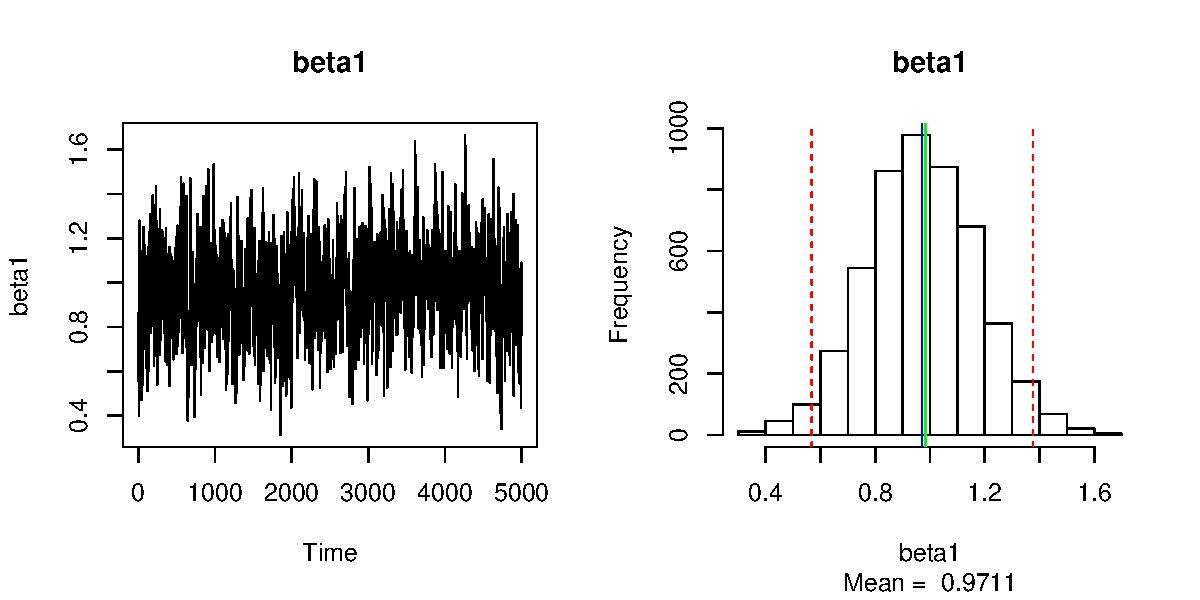
\includegraphics[scale = .7]{plot1.pdf} \\
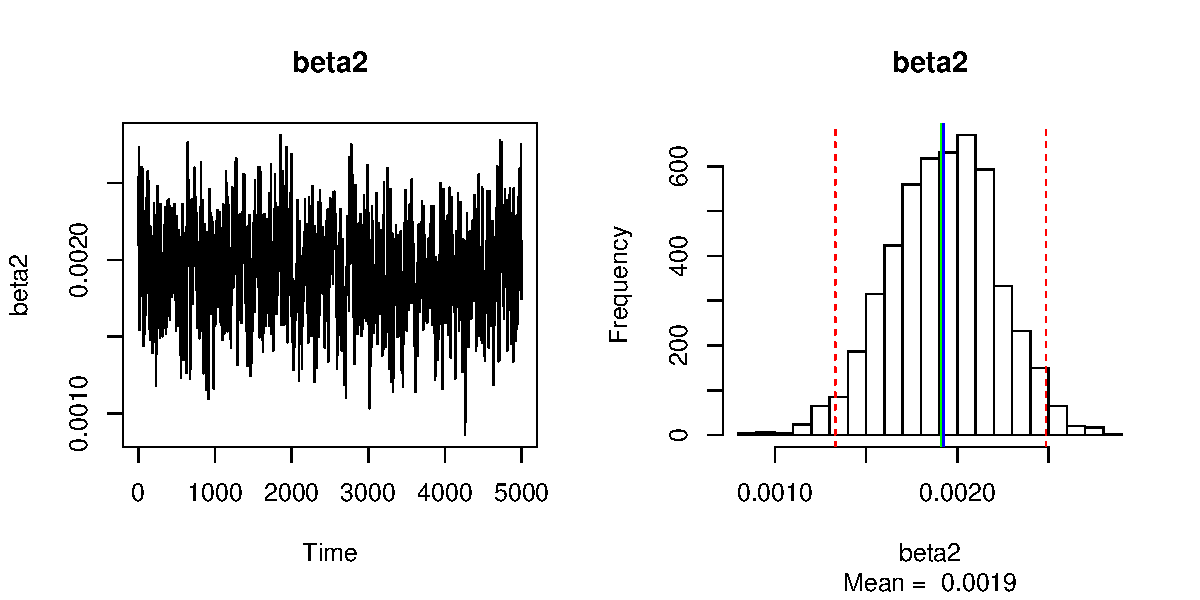
\includegraphics[scale = .7]{plot2.pdf} \\
\newline
Using these posterior estimates, we can generate point and interval estimates for the response mean. Those estimates are plotted below. with the blue points corresonding to the data, the black line the mean, and the red lines 95 percent confidence regions. \\
\newline
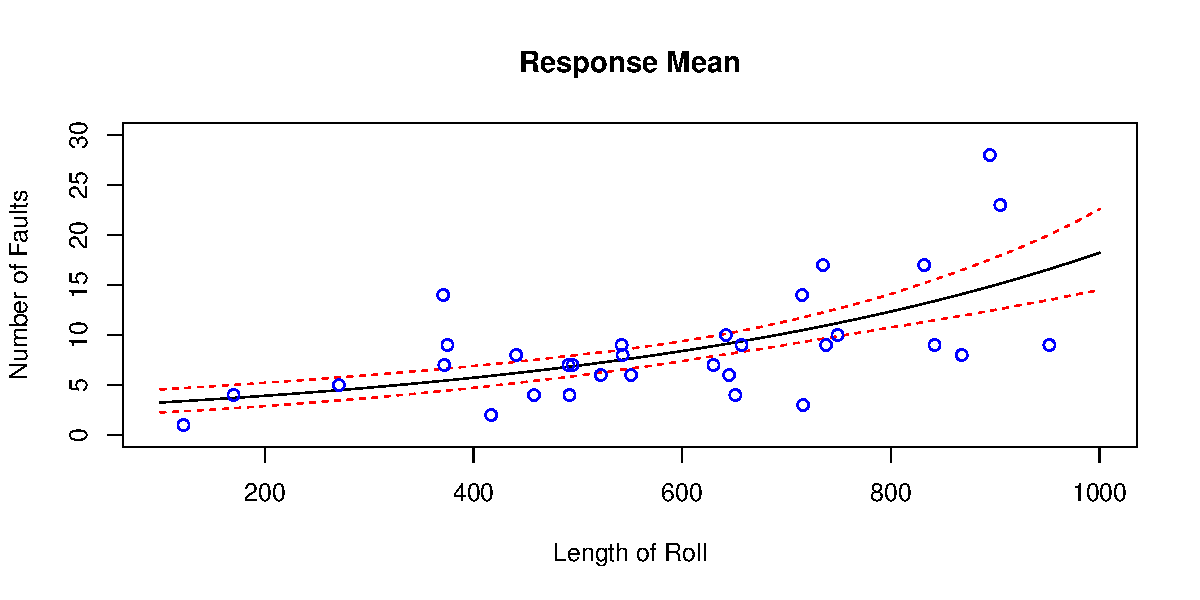
\includegraphics[scale = .7]{plot3.pdf} \\
\newline
Finally, we can take our posterior estimates of $\beta_1$ and $\beta_2$ and, for each fabric length in the data, generate a distribution of expected average numbers of faults. For each of these mean estimates, we then generate a random deviate from a poisson distribution. These random deviates are samples from the posterior predictive distribution. Subtracting the actual number of faults from this distribution gives us a distribution of posterior predictive residuals. We plot the 95 percent confidence regions for each data point in the plot below. Red indicates that zero is included in the region, while blue indicates the opposite. We note that six out of thirty two data points appear to be inconsistent with the model, which is much higher than one or two we might hope for with 95 percent confidence regions. \\
\newline
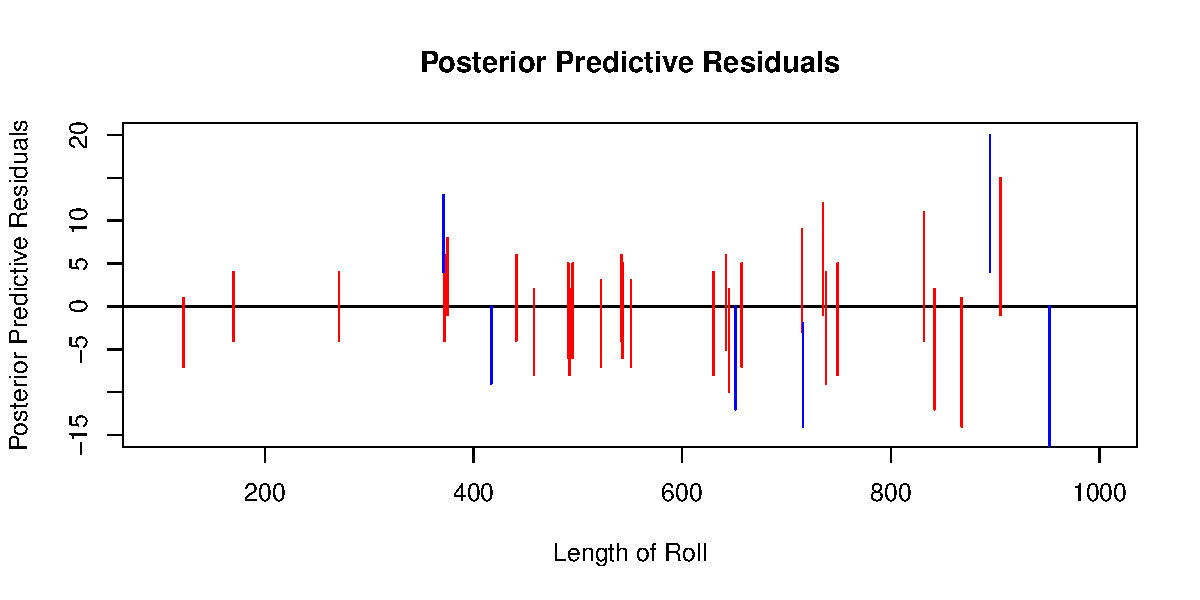
\includegraphics[scale = .7]{plot4.pdf} \\
\newline

\item In this problem, we explore a Bayesian Hierarchical Poisson GLM.  
\begin{enumerate}[(i)]
	\item Here we develop expressions for $E(Y_i| \beta_1, \beta_2, \lambda)$ and $Var(Y_i| \beta_1, \beta_2, \lambda)$ and compare them to the expressions in part (a). 
	\begin{align*}
	E(Y_i| \beta_1, \beta_2, \lambda) &= E^{\mu_i}(E(Y_i|\mu_i)) \\
	&= E^{\mu_i}(\mu_i) \\
	&= \gamma_i = exp(\beta_1 + \beta_2 x_i) \\
	Var(Y_i| \beta_1, \beta_2, \lambda) &= Var(E(Y_i|\mu_i)) + E(Var(Y_i|\mu_i))  \\
	&= Var(\mu_i) + E(\mu_i,) \\
	&= \frac{\gamma_i^2}{\lambda}+\gamma_i = exp(\beta_1 + \beta_2 x_i) + \frac{exp(\beta_1 + \beta_2 x_i)^2}{\lambda}
	\end{align*}
	Under the non-hierarchical model, $E(Y_i| \beta_1, \beta_2) = exp(\beta_1 + \beta_2 x_i)$, which is exactly the same. However, the variance is defined to be $Var(Y_i| \beta_1, \beta_2) = exp(\beta_1 + \beta_2 x_i)$ which we note is less than or equal to the variance of the hierarchical model. The variance of the hierarchical model is equal to the variance of the standard model only when $\lambda \rightarrow \infty$ which is the limiting case discussed in class, where the hierarchical GLM collapses to the standard GLM. 
	\item For our MCMC approach we use a Gibbs sampler with one normal update step for the $\mu_i$ and Metropolis Hastings for $\lambda$ and $\beta$ updates. The specific distributions that we use to compute the full posterior are detailed below. 
	\begin{align*}
	y_i|\mu_i &\sim Pois(\mu_i)  \\
	\mu_i|\gamma_i, \lambda &\sim Gamma(\lambda, \lambda\gamma^{-1}) \\
	p(\lambda) &= \frac{1}{(1+\lambda)^2} \\
	p(\beta) &\propto 1 \\
	log(\gamma_i) &= \beta_1 + \beta_2 x_i
	\end{align*}
	From the information above we can compute the full posterior and the corresponding full conditionals. This process is detailed below. 
	\begin{align*}
	p(\beta, \lambda, \mu|Y) &\propto p(Y|\beta, \lambda, \mu) p(\beta, \lambda, \mu) \\
	&= p(Y|\beta, \lambda, \mu)p(\mu|\lambda, \beta) p(\lambda)p(\beta) \\
	&= \bigg[\prod_{i=1}^{n}Pois(y_i|\mu_i)\bigg]\bigg[\prod_{i=1}^{n}Gamma(\mu_i|\lambda, \frac{\lambda}{\gamma_i})\bigg] \frac{1}{(1+\lambda)^2} *1 \\
	\mu_i|\cdot &\sim Gamma\bigg(\mu_i|y_i + \lambda, 1 + \frac{\lambda}{exp(\beta_1 + \beta_2 x_i)}\bigg)\\
	log(p(log(\lambda)|\cdot)) &\propto \sum_{i=1}^{n} \bigg[\lambda log\bigg(\frac{\lambda}{\gamma_i}\bigg) - log\Gamma(\lambda) +(\lambda - 1) log(\mu_i)- \lambda \mu_i \gamma_i^{-1}\bigg] - 2log(1 + \lambda)  + log(\lambda)\\
	log(p(\beta|\cdot)) &\propto \sum_{i=1}^{n} \bigg[-\lambda(\beta_1 + \beta_2 x_i) - \frac{\lambda \mu_i}{exp(\beta_1 + \beta_2 x_i)}\bigg]
	\end{align*}
	Using the above full conditionals, we implement a Gibbs Sampler. The $\mu_i$ sampling steps are easy, but for the MH steps, we have to generate candidates. MH requires the proposal distribution to be symmetric, but $\lambda >0$, so we make a change of variable to $log(\lambda)$ so we can sample from a normal distribution, which is symmetric. We then exponentiate our $log(\lambda)$ sample to get a lambda sample.   \\
	We generate beta candidates by sampling from a multivariate normal with diagonal covariance matrix. Under these proposal approaches, I ran the Gibbs Sampler for 300,000 iterations, and noted that it generally seemed to be converging to  ballpark values, but based on a time series plot of the samples of say $\beta_1$, didn't seem to be converging to a particular value. To try and improve the Gibbs Sampler performance, I took the mean $\lambda$ and $\mu_i$'s that were generated, and treated these as close enough to MLE values. I then maximized $log(p(\beta|\cdot))$ using these mean estimates as inputs to the non $\beta$ parameters of the log likelihood. The optim function in R gives a numerically approximated hessian, which I multiplied by -1 and took the inverse of to get a potentially better covariance matrix for candidate generation in the $\beta$ MH step.  Using this approach, I then reran the Gibbs sampler with fewer iterations to get the following posterior plots of $\beta_1$, $\beta_2$ and $\lambda$. \\
	\newline
	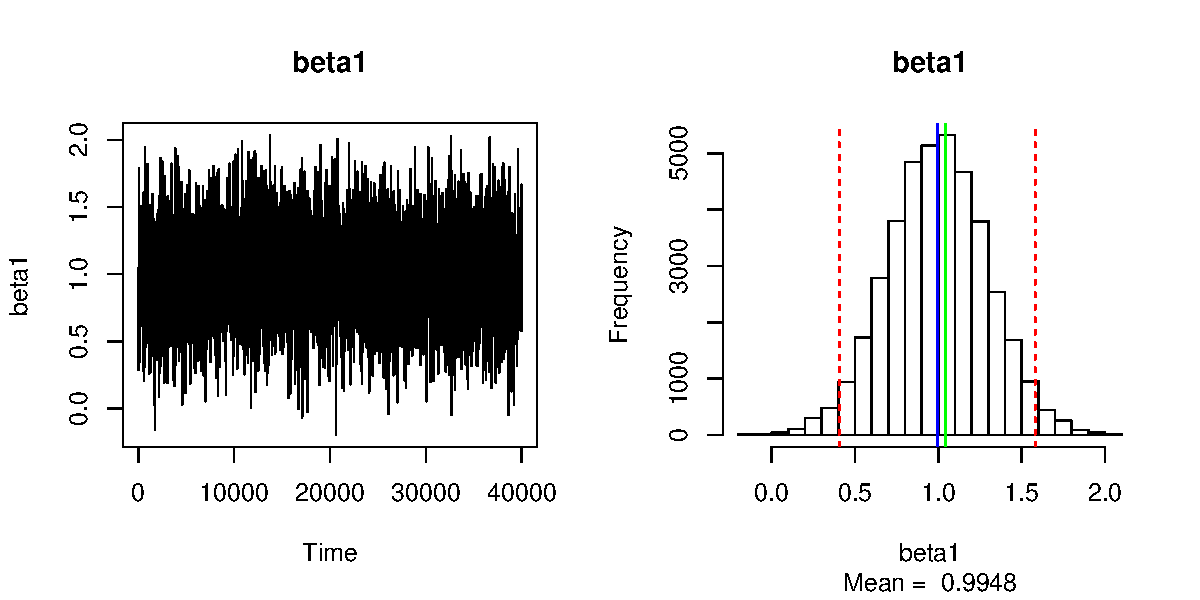
\includegraphics[scale = .7]{plot7.pdf} \\
	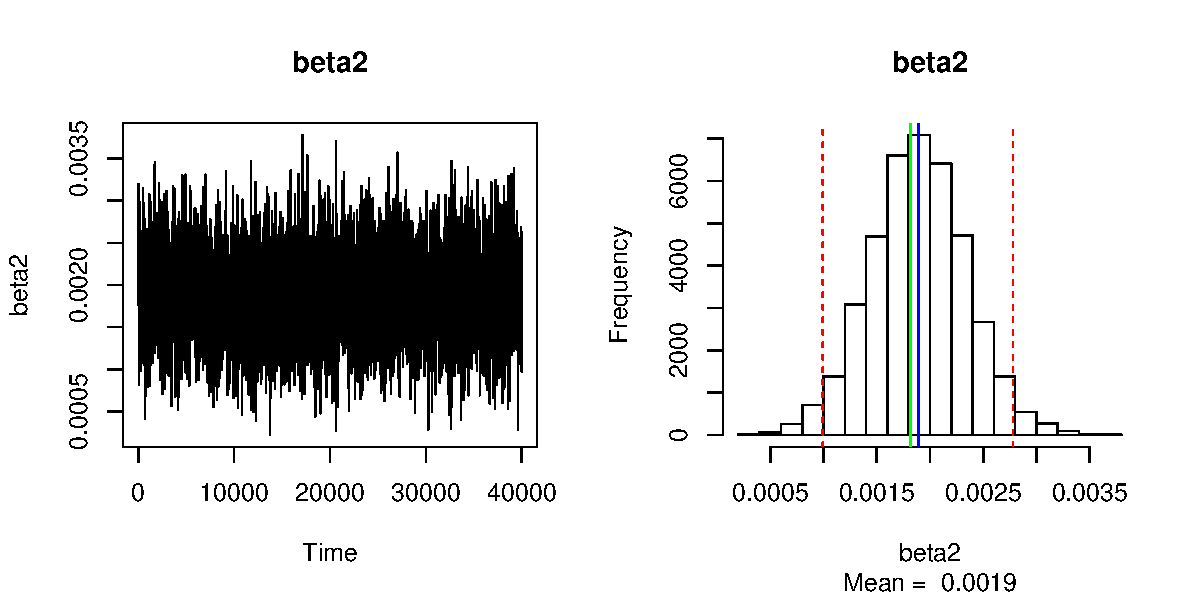
\includegraphics[scale = .7]{plot8.pdf} \\
	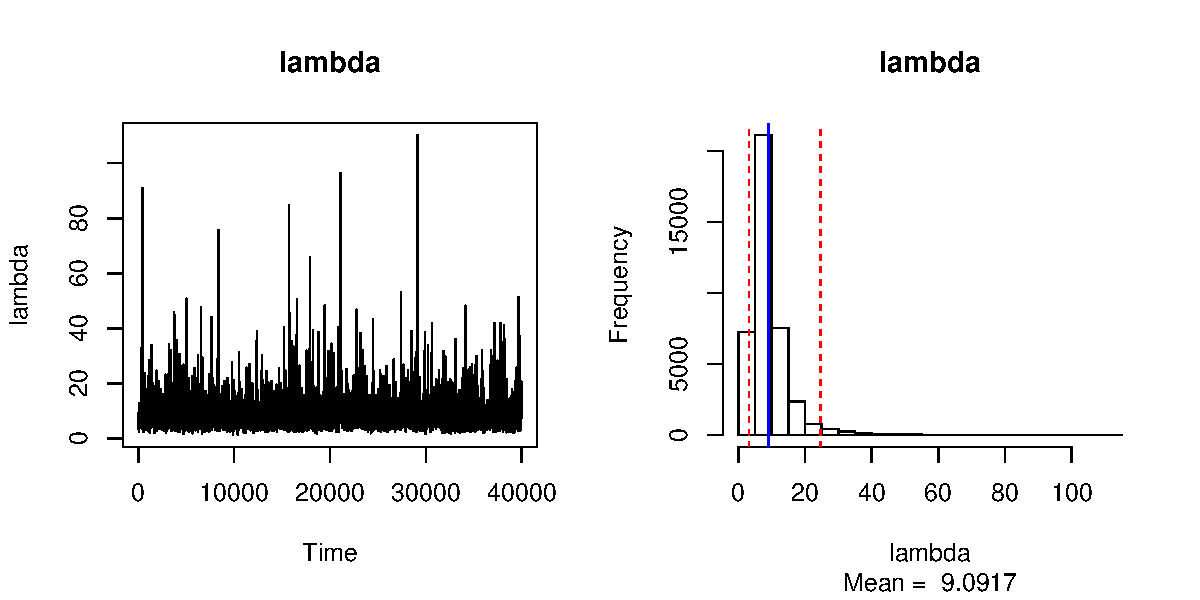
\includegraphics[scale = .7]{plot9.pdf} \\	
	\newline
	
	\item Next, we derive an expression for the posterior predictive distribution of a new unobserved response $y_0$ based on a new $x_0$. 
	\begin{align*}
	p(y_0|x_0, data) &= \int Pois(y_0|\mu_0)Gamma(\mu_0|\lambda, \lambda\gamma_0^{-1})p(\beta_1, \beta_2, \lambda|\textbf{y}) d\beta d\lambda d\mu_0\\
	&= \int \frac{e^{-\mu_0}\mu_0^{y_0}}{y_0!} \frac{(\lambda \gamma_0^{-1})^{\lambda}}{\Gamma(\lambda)}\mu_0^{\lambda -1} exp(-\lambda \gamma_0^{-1} \mu_0) p(\beta_1, \beta_2, \lambda|\textbf{y}) d\mu_0 d\beta d\lambda\\
	&= \int \frac{(\lambda \gamma_0^{-1})^{\lambda}}{\Gamma(\lambda)y_0!} \bigg[\int \mu_0^{y_0 + \lambda - 1} exp(-(\lambda \gamma_0^{-1} + 1) \mu_0) d\mu_0 \bigg]p(\beta_1, \beta_2, \lambda|\textbf{y})d\beta d\lambda\\
	&= \int \frac{(\lambda \gamma_0^{-1})^{\lambda}}{\Gamma(\lambda)y_0!} \frac{\Gamma(y_0 + \lambda)}{(\lambda \gamma_0^{-1} + 1)^{y_0 + \lambda}}p(\beta_1, \beta_2, \lambda|\textbf{y})d\beta d\lambda\\
	&= \int \frac{\Gamma(y_0+\lambda)}{\Gamma(y_0 - 1)\Gamma(\lambda)} \bigg(\frac{\lambda}{\lambda + \gamma_0}\bigg)^{\lambda}\bigg(\frac{\gamma_0}{\lambda + \gamma_0}\bigg)^{y_0} p(\beta_1, \beta_2, \lambda|\textbf{y})d\beta d\lambda\\ 
	&= \int NB\bigg(y_0|\lambda, \frac{\gamma_0}{\gamma_0 + \lambda}\bigg)p(\beta_1, \beta_2, \lambda|\textbf{y})d\beta d\lambda\\
	\text{where}\quad \gamma_0 &= exp(\beta_1 + \beta_2 x_0) 
	\end{align*}
	First, this distribution has no analytic form, but we can sample from it using our posterior samples.
	In particular, we can generate samples from the posterior predictive distribution by taking our posterior samples of $\beta_1, \beta_2$ and $\lambda$ and using those to sample directly from a negative binomial distribution to get samples of $y_0$. 
	\item 
	Next we use these posterior distributions to generate point and interval estimates for the response mean as a function of fabric length. As $E(Y_i|\gamma_i) = \gamma_i$ in this hierarchical GLM, the red lines correspond to a 95 percent confidence region of the $\gamma_i$, which we defined earlier as $\gamma_i = exp(\beta_1 + \beta_2x_i)$. That plot is included below, and we note that the mean curve is just about the same, but the confidence regions are substantially wider than the regions for the standard GLM.\\
	\newline
	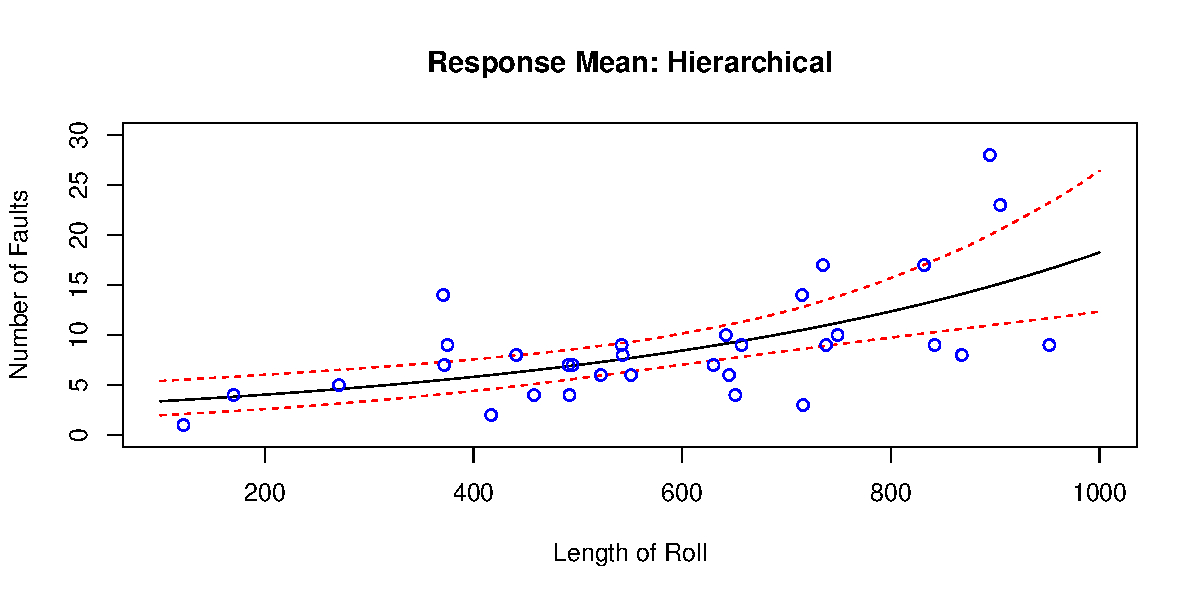
\includegraphics[scale = .7]{plot5.pdf} \\
	\newline
	\item Next we do some posterior predictive model checking. This time however, the $\mu_i$ are sampled for every MCMC iteration, rather than just $\beta_1, \beta_2$. So, in order to get posterior predictive replicate samples, we look at the following integral and note that we can generate posterior predictive samples of $y$ by taking random poisson samples with mean $\mu_i$, for each of the MCMC $\mu_i$ samples for data point i. 
	\begin{equation*}
	p(\hat{y}|y) = \int Poisson(\hat{y}|\mu_i) p(\mu_i|\textbf{y})d\mu_i
	\end{equation*}
	 This approach gives the following bayesian residual plot. Note that this time, every single observation has 0 as a possible value suggesting that this model is matching the data better than the standard GLM.\\
	 \newline
	 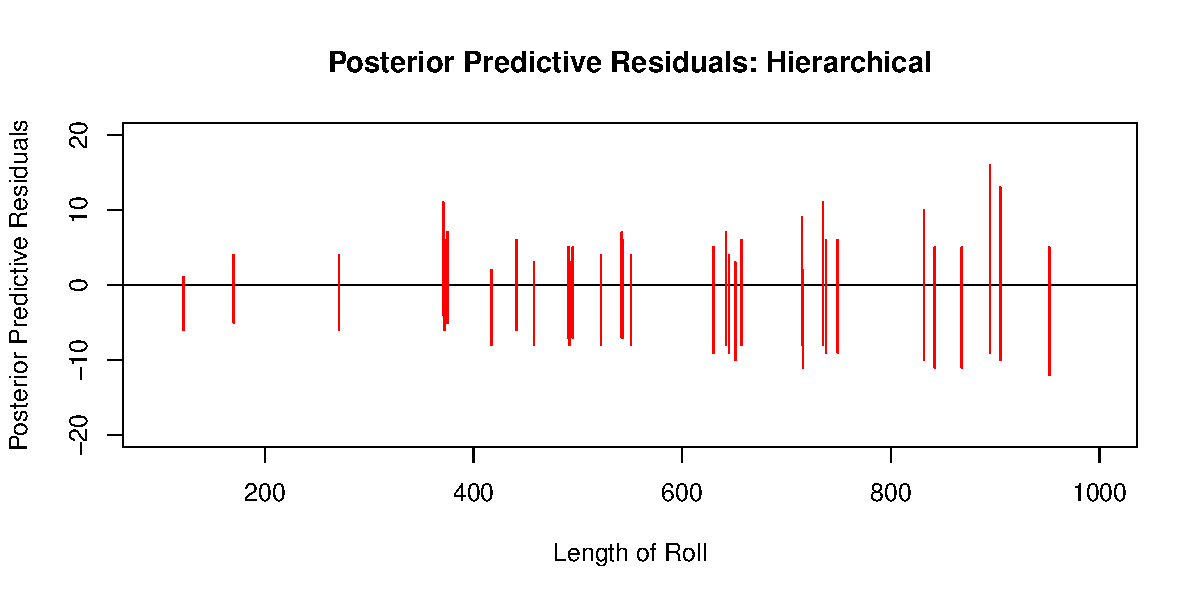
\includegraphics[scale = .7]{plot6.pdf} \\
	 \newline
	 \item Next we consider the sensitivity of our posterior to prior choice. In particular, we consider the following proper priors. Powers $p \leq 1$ aren't proper. 
	 \begin{align*}
	 p(\lambda) &= \frac{1}{(1+\lambda)^{p}}\\
	 p &\in \{1.01, 2, 10\}\\
	 p(\lambda) &= Gamma(.01, .01)
	 \end{align*}
	 These have plots below. We note that small p gives a lot of weight to large lambda values, while the gamma distribution doesn't have as much density for those values. \\
	 \newline
	 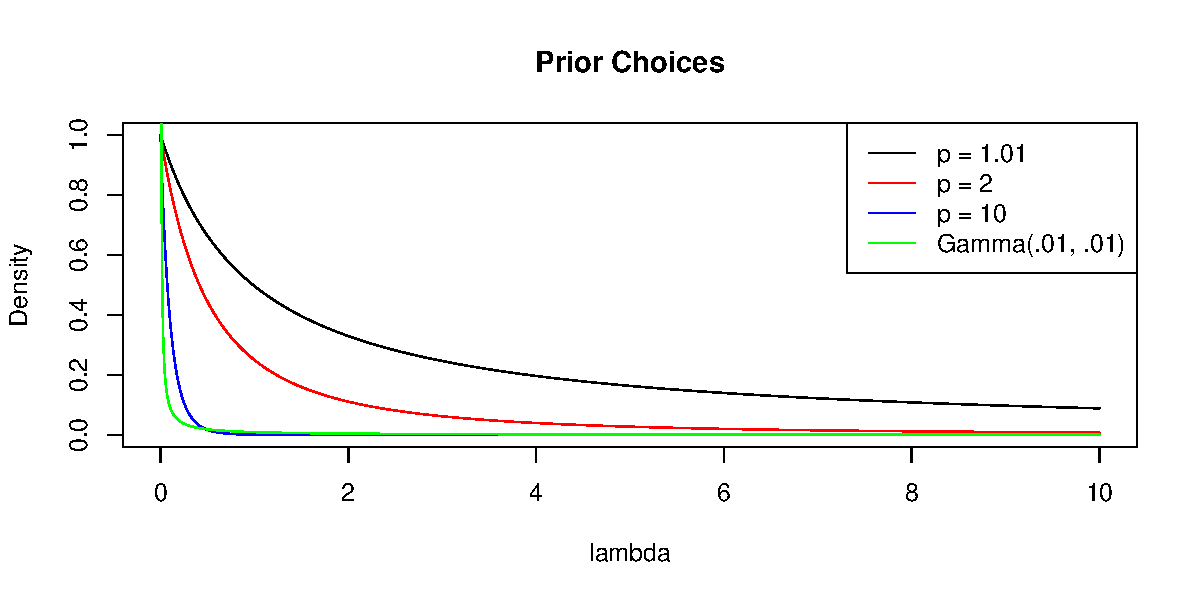
\includegraphics[scale = .7]{plot10.pdf}\\
	 \newline
	 We evaluate posterior sensitivity to prior specification first by looking at what the different priors do to posterior lambda estimates. The beta estimates remained fairly similar regardless of which lambda prior was used. \\
	 \newline
	 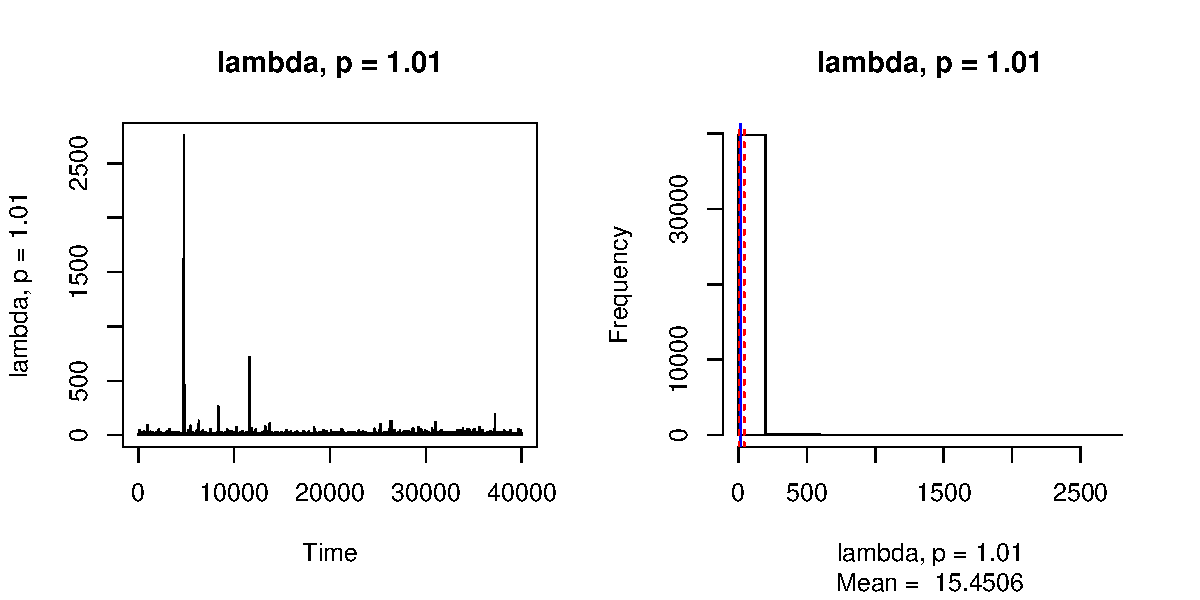
\includegraphics[scale = .7]{plot11.pdf}\\
	 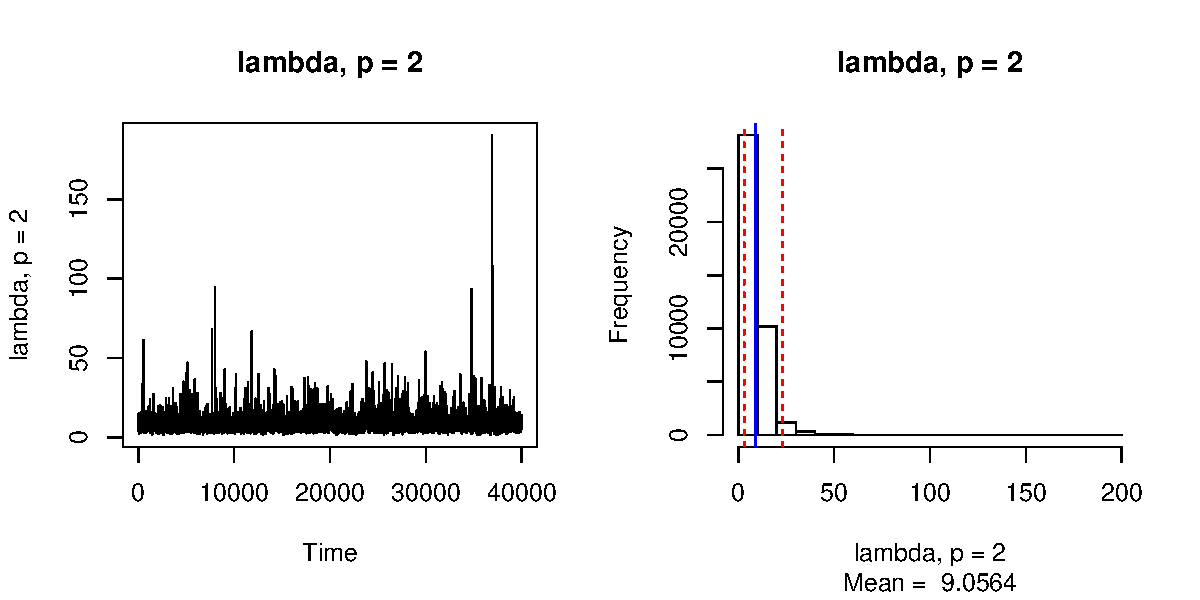
\includegraphics[scale = .7]{plot12.pdf}\\
	 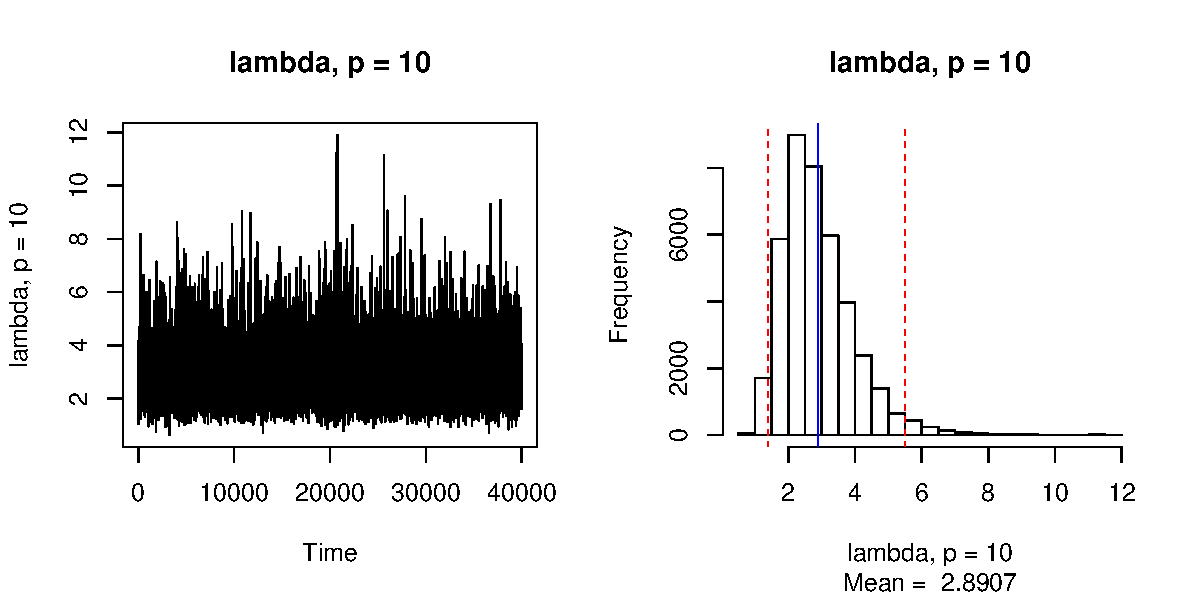
\includegraphics[scale = .7]{plot13.pdf}\\
	 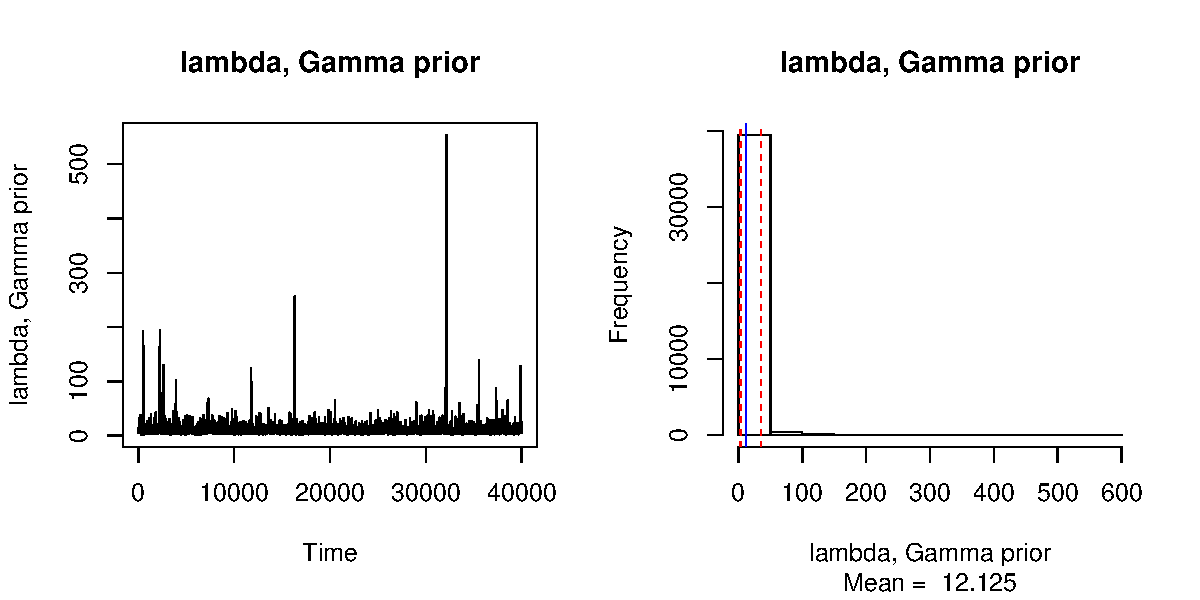
\includegraphics[scale = .7]{plot14.pdf}\\
	 \newline
	 Clearly, we see that lambda is highly affected by prior specification. To see how the different priors on lambda affect actual predictions of the $y_i$, we compute posterior predictive distributions based on new $x_0$'s over a grid. That approach yields the following plot. \\
	 \newline
	 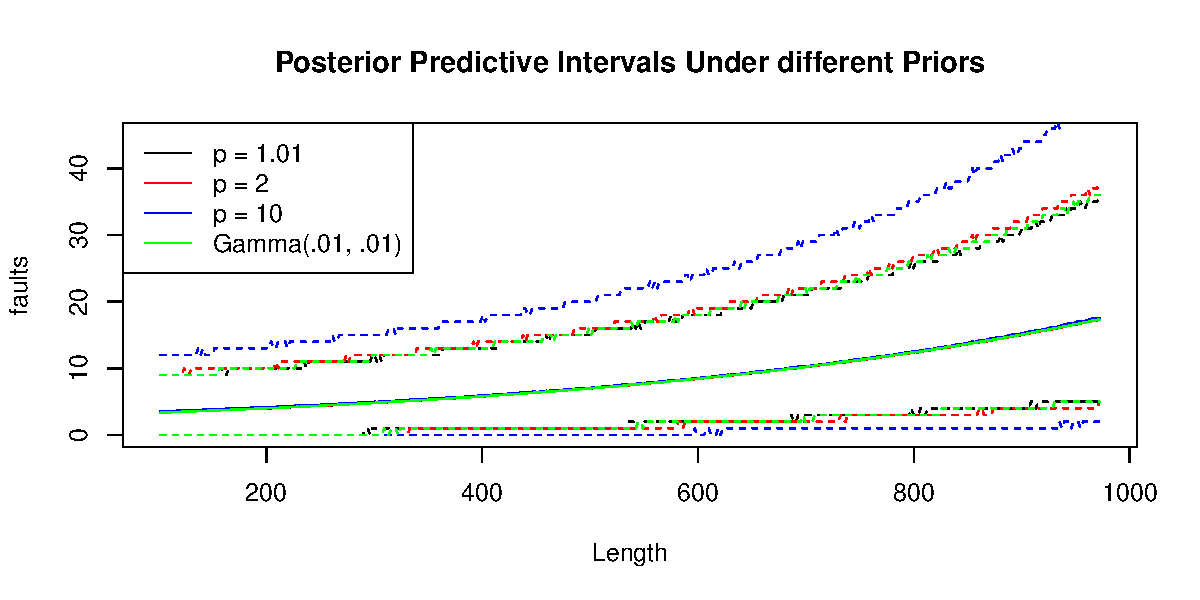
\includegraphics[scale = .7]{plot15.pdf}\\
	 \newline
	 We note that all priors produce posterior predictive distributions with relatively similar means. However the gamma, p = 2, and p = 1.01 produce posterior predictive distributions with similar spreads as well, while the p = 10 prior produces dramatically different confidence regions. This makes sense, as that prior enforces small lambdas. Lambda is a precision parameter, so with small lambda, we expect a model with that can accomodate a lot of overdispersion. This would cause the large confidence regions we see in the posterior predictive plot. 
	 
	 
	 
\end{enumerate}

\item Looking at our results from parts (a) and (b), it's clear that the hierarchical poisson model better models the data. In particular, we note that the 95 percent confidence regions of the posterior predictive bayesian residuals from the hierarchical GLM include zero for every replicate observation. In contrast, 6/32 observations on the standard GLM don't include zero. To better formalize the idea that the hierarchical model fits better, we compute the Gelfand and Ghosh predictive posterior loss criterion for both models, as well as for hierarchical models with different priors on $\lambda$. The Gelfand and Ghosh criteria is defined as follows, where $z_l$ are replicates of the data. 
\begin{align*}
\mu_l &= E(z_l|\textbf{x})\\
\sigma^2_l &= var(z_l|\textbf{x}) \\
G &= \sum_{l = 1}^{n} (\mu_l - x_l)^2  \\
P &= \sum_{l = 1}^{n} \sigma^2_l \\
D &= G + P 
\end{align*}


In order to get posterior samples of the $z_l$ in the hierarchical case, we generate samples from poisson distributions with means equal to our posterior mean samples. In the standard glm, we generate samples from a poisson distribution with $\mu = exp(\beta_1 + \beta_2 x)$ where x is some replicate data point, and the $\beta_i$ are posterior samples. We find that the hierarchical model fits the data much better, according to the Gelfand and Ghosh criterion. 


\begin{table}[]
	\centering
	\begin{tabular}{|l|l|l|l|}
		\hline
		Model            & G        & P        & D        \\ \hline
		Standard GLM     & 650.3489 & 302.8733 & 953.2222 \\ \hline
		Hierarchical GLM & 120.0659 & 456.2206 & 576.2865 \\ \hline
	\end{tabular}
\end{table}


Different priors on $\lambda$ drop the Gelfand and Ghosh criterion from around 576 to around 540, which is a small drop relative to the jump from the standard GLM. Because the criterion is relatively unaffected by prior choice, I didn't include the actual G, P and D values in the table above. 






	
\end{enumerate}

\end{document}